Für die Aufgabe wird grundsätzlich nur ein BMP benötigt.
Da wir uns jedoch entschieden haben, die Messdaten um Temperatur und Luftfeuchtigkeit zu erweitern, 
wird ein entsprechender zusätzlicher DHT mit eingebunden.

Da es die Sensoren für den ESP bereits auf entsprechenden Daughterboards angebracht gibt,
war es nur noch nötig diese aufzustecken:

\begin{figure}[h]
	\centering
	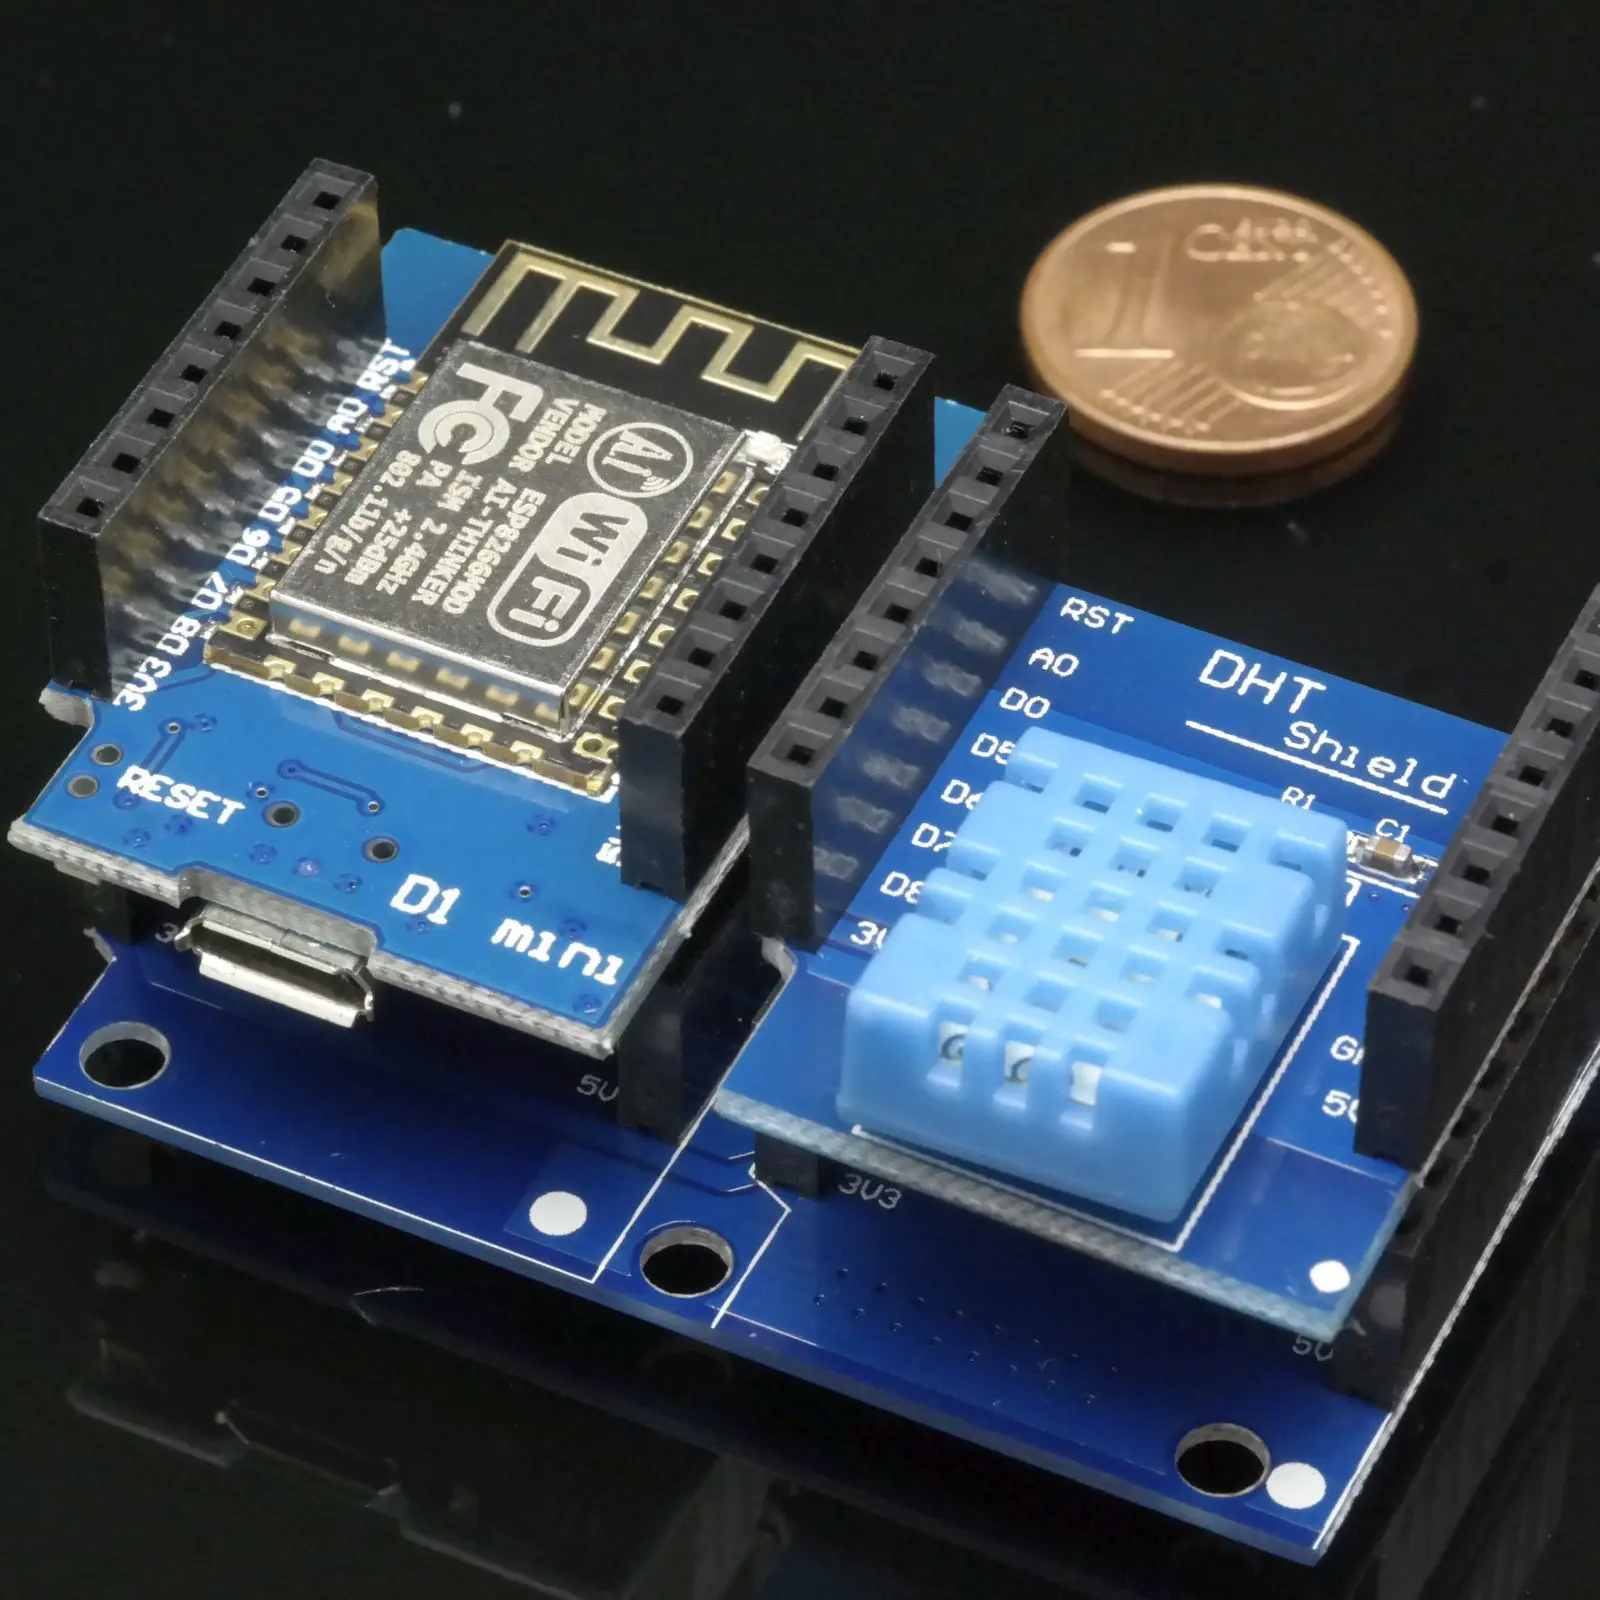
\includegraphics[width=7cm]{images/esp_dht.png}
	\caption[dht\_an\_esp]{DHT an ESP8266 angesteckt}
	\label{fig:dht_an_esp}
\end{figure}